\documentclass{HZNUMCM}
\setControlNumber{888888}
\setContestType{MCM}
\setProblemLetter{A}
\setPaperTitle{ A new $3/2$ type criteria on  global attractivity in a Logistic equation with piecewise constant arguments}
\setSummary{ This paper presents a new 3/2 type criteria of the form
$$\int_{n-m}^{n+1}r(t)dt-\exp\left(-\int_{n-m}^{n+1}r(t)dt-\frac{3}{2}\right)\leqslant \frac{3}{2}$$
 for the global attractivity of the positive steady state solution of the logistic equation with piecewise constant arguments
 $$\frac{dN(t)}{dt}=r(t)N(t)\left(1-\sum_{j=0}^{m}a_jN([t-j])\right),\quad t\geqslant 0,m\geqslant 0.$$
The new criteria improves the known results in literatures,including those proposed by Gopalsamy etal. \cite{1992_Gopalsamy}, So and Yu \cite{1995_so_MR1317052,1995_so_R1339824}.
Some results of computer simulations are given.
}

\begin{document}
\showSummarySheet
\showContents

\section{Introduction}
In this paper, we are concerned with a  study of the global attractivity of the positive steady state  solution of  the following logistic equation with piecewise constant arguments
\begin{equation}\label{logistic_equation}
\frac{dN(t)}{dt}=r(t)N(t)\left(1-\sum_{j=0}^{m}a_jN([t-j])\right),\qquad t\geqslant 0,m\geqslant0,
\end{equation}
where $[\cdot]$ denotes the greatest-integer function, $m$ is a fixed number,  $r(t)$ is a positive and continuous function on $[0,\infty)$  and
\begin{equation}\label{logistic_condition}
a_0,a_1,\cdots,a_{m}\geqslant 0, ~\sum_{i=0}^ma_i>0.
\end{equation}

By a solution of \eqref{logistic_equation} , we mean a function $N$ which is defined on the set
$$
\{-m,-m+1,\cdots,-1,0\}\cup(0,\infty),
$$ and satisfies the following properties:
\begin{itemize}
\item $N$ is continuous on $[0,\infty)$;
\item The derivative $\dot N(t)$ exists at each point $t\in [0,\infty)$ with the possible exception of the points $t\in\{0,1,2,\cdots\}$ where one-sided derivatives exist;
\item \eqref{logistic_equation} is satisfied on each interval $[n,n+1)$ where $n=0,1,2,\cdots$.
\end{itemize}

As claimed in  \cite{1995_so_R1339824} or \cite{1991_gopalsamy_MR1079622}, the equation \eqref{logistic_equation} together with initial conditions of the form
\begin{equation}\label{logistic_initial_condition}
N(0)=N_0>0 \text{~and~} N(-j)=N_{-j}\geqslant 0,\quad j=1,2,\cdots,m
\end{equation}
has a unique positive solution $N(t)$.


The only  positive steady state solution $N^*$ of \eqref{logistic_equation} and \eqref{logistic_condition} is
$$
N^*=1/\sum_{j=0}^ma_j.
$$



Above equations \eqref{logistic_equation}-\eqref{logistic_initial_condition} arise in some ecological applications. As one of special cases of equation \eqref{logistic_equation}, the delay differential equation
$$
y'(t)=r y(t) \left(1-\frac{x(t-\tau)}K\right),\quad t\geqslant 0,
$$
called the Hutchinson$'$s  equation \cite{NYAS:NYAS221}, was used by Hutchinson  to model the growth of a herbivore. Here $y(t)$ is the population of a single species at time $t$, $r$ is the intrinsic per capita growth rate of the population, $K>0$ is the carrying capacity of the habitat and $\tau>0$ is the time lag.  Some population model comes from Hutchinson$'$s equation.

Some other variant cases, such as
\begin{equation*}\label{case_eq}
y'(t)=r(t) y(t) \left(1-\frac{x([t])}K\right),\quad t\geqslant 0
\end{equation*}
has also been extensively discussed in the literatures, for instances,
\cite{1995_so_MR1317052,2008_li_MR2386489,2000_lyj_MR1770856,2001_ni_MR1881865,2011_Ozturk_1532,1995_so_R1339824,1992_Gopalsamy,2005_hu_MR2168581,2009_zhang_MR2537726,wxp_1999}
and the references cited therein.


Equation \eqref{logistic_equation} with the initial condition \eqref{logistic_initial_condition}  is  a more general form.
In this paper, we are interested in studying the sufficient conditions for the global attractivity of the positive steady state  solution of equations \eqref{logistic_equation} -\eqref{logistic_initial_condition} under the common assumption
\begin{equation}\label{common_condition}
\int_0^{\infty}r(t)dt=\infty.
\end{equation}

Before giving and proving our main results, let us state several classical studies on the global attractivity of the positive steady state solution of equations \eqref{logistic_equation} -\eqref{logistic_initial_condition}  and their some variant cases.


The first one is about the case where $r(t)\equiv r$($r$ is a
positive constant) and $m=0$. Early in 1955, Wright \cite{1955_Wright_MR0072363}  presented the following  conjecture.

 \vskip 0.2cm\noindent {\bf Conjecture A}. {\it In \eqref{logistic_equation}, if $r(t)\equiv r>0$ ($r$ is a constant), $m=0$ and
 $$r\leqslant\frac {\pi}{2},$$then the solution $N(t)$ of \eqref{logistic_equation}-\eqref{logistic_initial_condition}  tends to $N^*$ as $t\rightarrow\infty$.}

In 1992, Gopalsamy \cite{1992_Gopalsamy} showed  us a necessary  and sufficient condition for the global attractivity  of the positive steady state solution of \eqref{logistic_equation}-\eqref{logistic_initial_condition}  that
\vskip 0.2cm \noindent{\bf Theorem A}.
{\it Supposing $r(t)\equiv r>0$ and $m=0$, the solution $N(t)$ of \eqref{logistic_equation}-\eqref{logistic_initial_condition} tends to $N^*$ as $t\rightarrow\infty$ if and only if $$r \leqslant 2.$$
}

Obviously,   Theorem A confirmed Wright$'$s Conjecture A was right.

The second statement is about the case where $r(t)\equiv r$($r$ is a
positive constant) and for general $m\geqslant 0$.
In 1991, Gopalsamy etal \cite{1991_gopalsamy_MR1079622} proposed the following
\vskip 0.2cm \noindent{\bf Theorem B}.
{\it Assume $r(t)\equiv r>0$, $m\geqslant0$, and
\begin{equation}\label{go_condition}
r(m+1)<\log 2,
\end{equation} then the solution $N(t)$ of \eqref{logistic_equation}-\eqref{logistic_initial_condition}  tends to $N^*$ as $t\rightarrow\infty$.
}

Later, in 1992, Gopalsamy  \cite{1992_Gopalsamy}  proposed the following
 \vskip 0.2cm\noindent {\bf Conjecture B}. {\it In Theorem B, the condition \eqref{go_condition} may be replaced by
$$  r(m+1)e^{r(m+1)}<1.  $$}

The third statement is about the case where $r(t)$ is a positive and
continuous function on $[0,\infty]$.
In 1995, So and Yu \cite{1995_so_R1339824} showed the following Theorem C, which gives a $3/2$ type criteria for the
global attractivity  of the positive steady state solution of
 \eqref{logistic_equation}-\eqref{logistic_initial_condition}  with the general $m\geqslant 0$.
 \vskip 0.2cm \noindent {\bf Theorem C}.{\it Assume that $r(t)$  is positive and continuous function on $[0,\infty]$ such that \eqref{common_condition} holds, and that
\begin{equation}\label{so_condition}
\int_{n-m}^{n+1}r(t)dt\leqslant \frac 3 2, \quad m\geqslant 0,n\geqslant m,
\end{equation}then the solution $N(t)$ of \eqref{logistic_equation}-\eqref{logistic_initial_condition}  tends to $N^*$ as $t\rightarrow\infty$.
}

While in 2001, Matsunaga, Hara and Sakata \cite{2001_matsunaga_MR1828948} considered the special case $m=0$ and proved
 \vskip 0.2cm\noindent {\bf Theorem D}.
{\it Assume that
$r(t)$ is continuous and positive function on $[0,\infty)$ such that \eqref{common_condition} holds. If $m=0$  and
\begin{equation}\label{condition_m=0}
\int_{n}^{n+1}r(t)dt\leqslant 2,\quad n\geqslant 0,
\end{equation}then the solution $N(t)$ of \eqref{logistic_equation}-\eqref{logistic_initial_condition}  tends to $N^*$ as $t\rightarrow\infty$.
}
\begin{remark}
Clearly, if $r(t)$  is reduced to a constant $r>0$, then the sufficient conditon \eqref{condition_m=0}  in Theorem D can be changed the form  into the condition $r\leqslant 2$ of Gopalsamy$'$s Theorem A.
\end{remark}
\begin{remark}
If $r(t)$  is reduced to a constant $r>0$, then the sufficient condition \eqref{so_condition}  of Theorem C becomes
\begin{equation*}
r(m+1)\leqslant \frac 3 2,
\end{equation*} which is  weaker than \eqref{go_condition}.
\end{remark}

Additionally, by comparing the forms of above conditions with the form of condition $r\leqslant{\pi/2}$ in Wright$'$s Conjecture A, the following question A is raised  naturally.


 \vskip 0.2cm\noindent {\bf
Question A}.{
{ Is that $$r(m+1)\leqslant{\frac{\pi}{2}}
$$ a sufficient condition  for the global attractivity of the positive steady state solution of \eqref{logistic_equation}-\eqref{logistic_initial_condition} when $m\geqslant0$?}
}
 \vskip 0.2cm
 The following counter-example shows that the answer to Question A is ``No"!  Let us choose
\begin{align*}
&m=2000,\\
&N(-2000)=N(-1999)=\cdots=N(-1)=N(0)=1.001,\\
&a_0=a_1=\cdots=a_{m-1}=0,a_m=1,\\
&r=\pi/(2(m+1))=\pi/4002
\end{align*}in  \eqref{logistic_equation}-\eqref{logistic_initial_condition}.  Figure \ref{fig0} shows the computer simulation result, which stands for the diagram of the solution $N(t)$ with respect to $t$. From Figure \ref{fig0}, we know the solution $N(t)$ is divergent, which shows us that $\pi/2$ is a can-not-reached up-bound of $r(m+1)$ for the solution of \eqref{logistic_equation}-\eqref{logistic_initial_condition} to be attracted under the situation $m\geqslant 0$.
\begin{figure}[htbp]
\begin{center}
 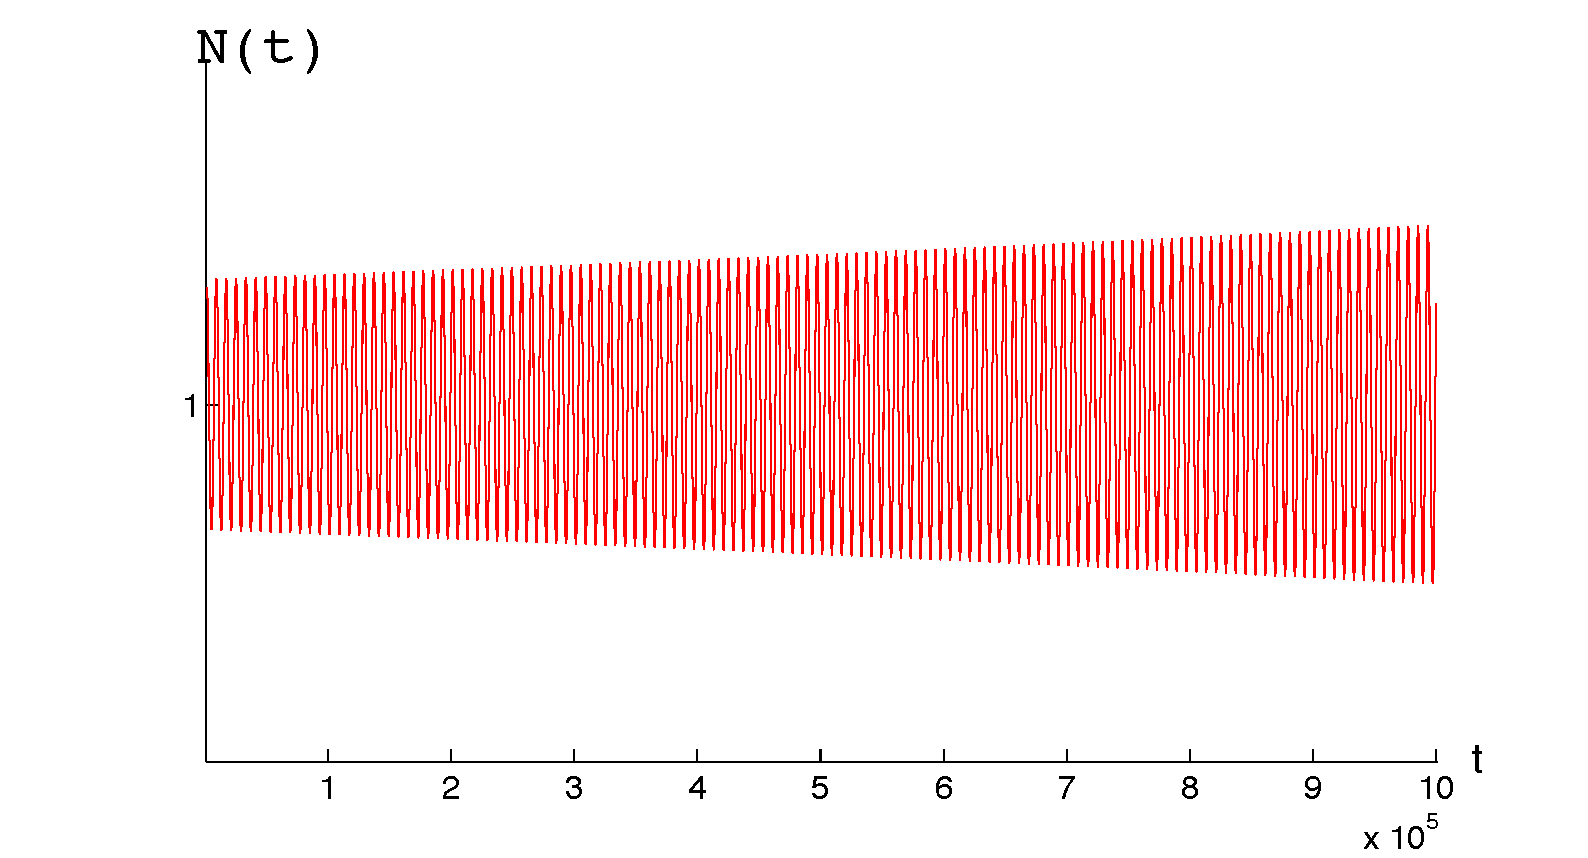
\includegraphics[width=\textwidth]{nt.pdf}
 \caption{The solution $N(t)$ of a counter-example. }\label{fig0}
 \end{center}
\end{figure}

Of course, after 2001,  researchers go on  keeping hard work for the study of the sufficient condition for the global attractivity of the solution of a logistic equation especially with piecewise constant arguments.

In 2003, Muroya \cite{2003_muroya_MR1962027} proposed  another type of sufficient condition for the global attractivity  of the solution of \eqref{logistic_equation} with \eqref{logistic_initial_condition}:
\begin{equation}\label{eq_2003}
a_0>\sum_{j=1}^ma_j\geqslant0\text{~~and~~}0<\inf_{l\geqslant0}r_l\leqslant r_l\leqslant 1,\quad l=0,1,2,\cdots,
\end{equation}
where $r_l=\int_l^{l+1}r(t)dt,l=0,1,2,\cdots$.
And from then on, this kind of conditions like \eqref{eq_2003} focusing on the relations among the coefficients  $a_j,j=0,1,2,\cdots,m$ has been investigated, such as  \cite{2009_li_R2451705,2008_muroya_MR2428273,2009_muroya_MR2481600,2010_nakata_MR2680013,2011_Ozturk_1532,2005_uesugi_MR2061343}.


But by now, based on the literatures as we knew, So and Yu$'$s result (Theorem C) maybe  the best one for  the solution of \eqref{logistic_equation}-\eqref{logistic_initial_condition} to be attracted under the situation that $r(t)>0$ is a continuous function and $m\geqslant 0$ without considering the relations among the coefficients  $a_j,j=0,1,2,\cdots,m$.  And then, an other question appears naturally.
 \vskip 0.2cm\noindent {\bf
Question B}. {Does there exist a more weaker sufficient condition than the one So and Yu  \cite{1995_so_R1339824} proposed, or say the one in  Theorem C for the global attractivity of the solution $N(t)$ for  \eqref{logistic_equation}-\eqref{logistic_initial_condition}without considering any relation among the coefficients $a_j, j=0,1,\cdots,m$?}
 \vskip 0.2cm
It is just the main aim for this paper to study. By lots of computer simulations, we find that the answer to Question B  should be ``Yes".
 We find a larger than $3/2$ and can-reached ``up-bound" of $r(m+1)$ for  the solution $N(t)$ of \eqref{logistic_equation}-\eqref{logistic_initial_condition} to be attracted under the situation $m\geqslant 0$ and generalize our discovery  to fit for the situation where $r(t)$ is a positive and continuous function on $[0,\infty)$.  Our discovery is also inspired by So and Yu \cite{1995_so_R1339824}. We prove our results mainly by the properties of nonlinear convex functions and by the means of Taylor$'$s formula. The results we get improve the one  So and Yu \cite{1995_so_R1339824} proposed, for the global attractivity of the solution of \eqref{logistic_equation}-\eqref{logistic_initial_condition}  without considering any relation among the coefficients $a_j, j=0,1,\cdots,m$.

The rest of the paper is organized  as follows. In section 2, we present our main results. In section 3, we give the proofs. In section 4, we list some computer simulations.

\section{Main results}
In this section, we give our main results:
\begin{theorem}\label{ourcondition}
Assume that
\begin{equation}\label{ourcondition_eq}
\int_{n-m}^{n+1}r(t)dt-\exp\left(-\int_{n-m}^{n+1}r(t)dt-\frac 3 2\right)\leqslant\frac 3 2,\quad n\geqslant m\end{equation}
and \eqref{common_condition} hold, then the solution $N(t)$ of \eqref{logistic_equation} and \eqref{logistic_condition}  with the initial conditions \eqref{logistic_initial_condition} satisfies
$$
\lim_{t\rightarrow\infty}N(t)=N^*.
$$
\end{theorem}
\begin{remark}
By comparing \eqref{so_condition} with \eqref{ourcondition_eq}, we confirm that the answer to Question B in Section 1 is ``Yes"!.
\end{remark}

\begin{corollary}\label{cor1}
Assume that $r(t)\equiv r>0$ is a constant in \eqref{logistic_equation}, and
\begin{equation}\label{ourcondition_eq_r}
r(m+1)-e^{-r(m+1)-1.5}\leqslant\frac 3 2
\end{equation}
holds, then the solution $N(t)$ of \eqref{logistic_equation} and \eqref{logistic_condition}  with the initial conditions \eqref{logistic_initial_condition}  tends to $N^*$ as $t\rightarrow\infty$.
\end{corollary}



\section{Proofs of Theorem}
In this section, we will prove Theorem \ref{ourcondition}. Before the proof, we need some lemmas.

\begin{lemma}\label{lowbound}
For $k \in [0,1]$, $x \in [x_a,x_b]$  with $x_a=0$ and $x_b$ satisfying
\begin{equation*}
1.5 + e^{-x_b-1.5} - x_b=0,
\end{equation*}
 it holds
\begin{equation}\label{inequality_lowbound}
x (1 - e^{-k (1.5 + e^{-x-1.5} - x)})\leqslant k - k^2/3.
\end{equation}
\end{lemma}
\begin{proof}Let
$$
p(x) := x  (1.5 + e^{-x-1.5} - x),\qquad x\in[x_a,x_b],
$$ we know that
\begin{equation}\label{px}
\begin{split}
&p(x_a)=p(x_b)=0,\\
&p'(x)= 1.5+e^{-1.5-x}-x-x(1+e^{-1.5-x}) \\
&p'(x_a)=p'(0)=1.5+e^{-1.5-0}-0-0(1+e^{-1.5-0})>1.5 >0,\\
&p'(x_b)=-(1 + e^{-x_b-1.5}) x_b<0
\end{split}
\end{equation}and
\begin{equation}\label{dpx}
p''(x)=-2+(x-2)e^{-x-1.5}<0,
\end{equation}
for $x\in[x_a,x_b], $since $x\leqslant x_b<2$ by the condition.

\eqref{px} and \eqref{dpx} show $p(x)$ has a unique maximum in$[x_a,x_b]$. In fact,  since $0<e^{-2.27}<0.11$ deduce to
\begin{equation}
\begin{split}
p'(0.77)&=  1.5 + e^{-1.5-0.77} -0.77-0.77(1+e^{-1.5-0.77} )\\
&= 1.5 + e^{-2.27} -0.77-0.77-0.77e^{-2.27} \\
&=-0.04+0.23e^{-2.27}\\
&\leqslant-0.04+0.23\times 0.11=-0.0147<0,
\end{split}\end{equation}
and for every $x\in [x_a,x_b]$, $\exists\xi\in(0.77,x)\mbox{~or~}\xi\in(x,0.77)$, we have
\begin{equation} \label{px<0.66}
\begin{split}
p(x)&=p(0.77)+p'(0.77)(x-0.77)+p''(\xi){(x-0.77)^2}/2\\
&\leqslant p(0.77)+p'(0.77)(x-0.77)\\
&= 0.77 (1.5 + e^{-2.27} -0.77)+(x-0.77)p'(0.77))\\
&= 0.77 (1.5 + e^{-2.27} -0.77)+x p'(0.77)-0.77p'(0.77)\\
&\leqslant  0.77 (1.5 + e^{-2.27} -0.77) -0.77 p'(0.77)\\
&= 0.77 (1.5 + e^{-2.27} -0.77)+0.77(0.04-0.23e^{-2.27} )\\
&= 0.77 (1.5 + e^{-2.27} -0.77+0.04-0.23e^{-2.27} )\\
&= 0.77 (1.5  -0.77+0.04+0.77e^{-2.27} )\\
&\leqslant 0.77 (1.5 - 0.77 + 0.04 + 0.77 \times 0.11)=0.658119<0.66
\end{split}\end{equation}
by Taylor$'$s formula,


For $k\in[0,1]$, by \eqref{px<0.66}, it obviously  holds
$$p(x)\leqslant 1-\frac k 3,\qquad x\in [x_a,x_b],$$
which deduces to
$$
k p(x)\leqslant k-k^2/3,\qquad k\in[0,1],x\in[x_a,x_b]
$$
and
$$
-k p(x)\geqslant -(k-k^2/3),\qquad k\in[0,1],x\in[x_a,x_b].
$$

Clearly, if $k=0$ or $x=0$, then \eqref{inequality_lowbound} holds. So, we assume that $k\neq 0$ and $x\neq0$ in the following discussion.

So,
$$
\frac{-k p(x)}{x}=-k(1.5+e^{-x-1.5}-x)\geqslant \frac{-(k-k^2/3)}{x},\qquad k\in(0,1],x\in(x_a,x_b].
$$
which means
\begin{equation}\label{eq111}
1-k(1.5+e^{-x-1.5}-x)\geqslant 1-\frac{(k-k^2/3)}{x},\qquad k\in(0,1],x\in(x_a,x_b].
\end{equation}
Because of $$e^{X}\geqslant 1+X,\qquad X\in\mathbb R,$$
we have
$$e^{-k(1.5+e^{-x-1.5}-x)}\geqslant 1-k(1.5+e^{-x-1.5}-x),\qquad k,x\in\mathbb R.$$
Then, by \eqref{eq111},
$$e^{-k(1.5+e^{-x-1.5}-x)}\geqslant  1-\frac{(k-k^2/3)}{x},\qquad k\in(0,1],x\in(x_a,x_b],$$
which shows
$$1-e^{-k(1.5+e^{-x-1.5}-x)}\leqslant  \frac{(k-k^2/3)}{x},\qquad k\in(0,1],x\in(x_a,x_b],$$

Thus,
\begin{equation}\label{kleq0.4}
x(1-e^{-k(1.5+e^{-x-1.5}-x)})\leqslant  k-k^2/3,\qquad k\in(0,1],x\in(x_a,x_b]
\end{equation}holds.

The proof is completed.
\end{proof}






\begin{lemma}\label{upbound0.8}
For  $x \in [x_a,x_b]$  with $x_a=0$ and $x_b$ satisfying
\begin{equation*}
1.5 + e^{-x_b-1.5} - x_b=0,
\end{equation*}
 it holds
\begin{equation}\label{inequality_upbound0.8}
x (e^{0.5 (1.5 + e^{-x-1.5} - x)}-1)\leqslant0.5
\end{equation}
and
\begin{equation}\label{inequality_upbound1.31}
x (e^{ 1.5 + e^{-x-1.5} - x}-1)\leqslant  \frac{4}3.
\end{equation}
\end{lemma}
\begin{proof}
1) Let$'$s prove \eqref{inequality_upbound0.8} first. It is clearly right if $x=0$. So, it is needed us to prove \eqref{inequality_upbound0.8} only for $x\neq 0$. We assume $x\in(0,x_b]$ in the followings.

Let $$\phi(x)=e^{-0.5(1.5 + e^{-x-1.5} - x)},$$
then $$\phi'(x)=0.5 e^{-0.5 \left(1.5 +e^{-1.5-x}-x\right)} \left(1+e^{-1.5-x}\right)
$$
and
\begin{align*}
\phi''(x)&=e^{-0.5 \left(1.5 +e^{-1.5-x}-x\right)} (-0.5 e^{-1.5-x}+0.25 \left(1+e^{-1.5-x}\right)^2)\\
        &= e^{-0.5 \left(1.5 +e^{-1.5-x}-x\right)}(-0.5 e^{-1.5-x}+0.25(1+2 e^{-1.5-x}+( e^{-1.5-x})^2))\\
        &=e^{-0.5 \left(1.5 +e^{-1.5-x}-x\right)}e^{-1.5-x}(-0.5+0.25((e^{1.5+x})+2 +e^{-1.5-x}))\\
        &\geqslant e^{-0.5 \left(1.5 +e^{-1.5-x}-x\right)}e^{-1.5-x}(-0.5+0.25(e^{1.5})+2+0)> 0,
\end{align*}which means $\phi(x)$ is a convex function and by Taylor$'$s formula, for $x\in(0,x_b]$, we get

\begin{equation}\label{l1}
\begin{split}
\phi(x)&= \phi(0.7)+\phi'(0.7)(x-0.7)+\frac{\phi''(\xi)(x-0.7)^2}2\\
&\geqslant \phi(0.7)+\phi'(0.7)(x-0.7)\\
&=e^{-0.5(0.8 + e^{-2.2} )}+0.5 e^{-0.5 \left(0.8 +e^{-2.2}\right)} \left(1+e^{-2.2}\right)(x-0.7)\\
&=e^{-0.5(0.8 + e^{-2.2} )}(1+0.5 \left(1+e^{-2.2}\right)(x-0.7))\\
&=e^{-0.5(0.8 + e^{-2.2} )}(1-0.35 \left(1+e^{-2.2}\right)+0.5 \left(1+e^{-2.2}\right)x)=:l_1(x),
\end{split}
\end{equation}where $\xi\in[0.7,x] \text{~or~} \xi\in[x,0.7]$.

Now, let
$$
\psi(x)=\frac x {x+0.5},
$$then
$$
\psi'(x)=-\frac{x}{(0.5 +x)^2}+\frac{1}{0.5 +x}
$$
and
$$
\psi''(x)=\frac{2}{(0.5 +x)^2}\left(\frac{x}{0.5+x}-1\right)<0,
$$
which deduces to
\begin{equation}\label{l2}
\begin{split}
\psi(x)&=\psi(0.7)+\psi'(0.7)(x-0.7)+\frac{\psi''(\xi)(x-0.7)^2}2\\
&\leqslant \psi(0.7)+\psi'(0.7)(x-0.7)\\
&=\frac{0.7}{1.2}+\left(-\frac{0.7}{(0.5 +0.7)^2}+\frac{1}{0.5 +0.7}\right)(x-0.7)\\
&=\frac{0.7}{1.2}+\frac{0.5}{1.44}(x-0.7)\\
&=\frac{0.49}{1.44}+\frac{0.5}{1.44}x=:l_2(x),
\end{split}
\end{equation}where $\xi\in[0.7,x] \text{~or~} \xi\in[x,0.7]$
by Taylor$'$s formula too.

Then, by \eqref{l1}, \eqref{l2}, $e^{-0.4555}>0.63$ and  $0.11<e^{-2.2}<0.111$,  we can check
\begin{equation}\label{l1-l2at0}
\begin{split}
l_1(0)-l_2(0)&=e^{-0.5(0.8 + e^{-2.2} )}(1-0.35 \left(1+e^{-2.2})\right)-\frac{0.49}{1.44}\\
&> e^{-0.5(0.8 + e^{-2.2} )}(1-0.35 \times 1.111)-\frac{0.49}{1.44}\\
&> e^{-0.5(0.8 +0.111 )}(1-0.35 \times 1.111)-\frac{0.49}{1.44}\\
&= e^{-0.4555}0.61115-\frac{0.49}{1.44}\\
&> 0.38-0.35>0\\
\end{split}
\end{equation}
and
\begin{equation}\label{l1-l2at1.7}
\begin{split}
l_1(1.7)-l_2(1.7)&=e^{-0.5(0.8 + e^{-2.2} )}(1+0.5 \left(1+e^{-2.2})\right)-\frac{0.49+0.85}{1.44}\\
&> e^{-0.5(0.8 + e^{-2.2} )}(1+0.5 \times 1.11)-\frac{1.34}{1.44}\\
&> e^{-0.5(0.8 +0.111 )}(1+0.5 \times 1.11)-\frac{1.34}{1.44}\\
&= e^{-0.4555}1.555-\frac{1.34}{1.44}\\
&= 0.63\times1.555-\frac{1.34}{1.44}\\
&> 0.97-0.94>0.
\end{split}
\end{equation}


By \eqref{l1-l2at0}, \eqref{l1-l2at1.7} and the fact that $l_1(x),l_2(x)$ are two lines, we get
\begin{equation}\label{l1<l2}
l_1(x)>l_2(x),\qquad x\in[0,1.7].
\end{equation}

Combining \eqref{l1<l2} with  \eqref{l1} , \eqref{l2} and the fact $x_b<1.7$, we have
$$
\phi(x)\geqslant l_1(x)> l_2(x)\geqslant\psi(x),\qquad x\in(0,x_b],
$$
which leads to
$$
\phi(x)=e^{-0.5(1.5 + e^{-x-1.5} - x)}>\frac{x}{0.5+x}=\psi(x),\qquad x\in(0,x_b],
$$then
$$
e^{0.5(1.5 + e^{-x-1.5} - x)}<\frac{0.5}{x}+1,\qquad x\in(0,x_b],
$$
which shows \eqref{inequality_upbound0.8} holds for $x\in (0,x_b]$. Since \eqref{inequality_upbound0.8} holds for $x=0$ as we claimed before, the proof of the first part is completed.

\noindent 2) We use the similar method as we did in the first part to  prove the second part. It suffices to prove
\begin{equation}\label{targetineq}
e^{-(1.5 + e^{-x-1.5} - x)}>\frac{x}{4/3+x},\qquad x\in(0,x_b].
\end{equation}
Let $$\Phi(x)=e^{-(1.5 + e^{-x-1.5} - x)},\qquad x\in(0,x_b]$$
then $$\Phi'(x)= e^{-\left(1.5 +e^{-1.5-x}-x\right)} \left(1+e^{-1.5-x}\right),\qquad x\in(0,x_b]
$$
and
\begin{align*}
\Phi''(x)&=e^{- \left(1.5 +e^{-1.5-x}-x\right)} (- e^{-1.5-x}+ \left(1+e^{-1.5-x}\right)^2)\\
        &= e^{- \left(1.5 +e^{-1.5-x}-x\right)}(- e^{-1.5-x}+(1+2 e^{-1.5-x}+( e^{-1.5-x})^2))\\
        &=e^{- \left(1.5 +e^{-1.5-x}-x\right)}e^{-1.5-x}(-1+((e^{1.5+x})+2 +e^{-1.5-x}))\\
        &\geqslant e^{- \left(1.5 +e^{-1.5-x}-x\right)}e^{-1.5-x}(-1+(e^{1.5})+2+0)> 0,
\end{align*}which means $\Phi(x)$ is a convex function. Then  by Taylor$'$s formula, for every $x\in(0,x_b]$, we get
\begin{equation}\label{L1}
\begin{split}
\Phi(x)&= \Phi(0.54)+\Phi'(0.54)(x-0.54)+\frac{\Phi''(\xi)(x-0.54)^2}2\\
&\geqslant \Phi(0.54)+\Phi'(0.54)(x-0.54)\\
&=e^{-(0.96 + e^{-2.04} )}+e^{- \left(0.96 +e^{-2.04}\right)} \left(1+e^{-2.04}\right)(x-0.54)\\
&=e^{-(0.96 + e^{-2.04} )}(1+ \left(1+e^{-2.04}\right)(x-0.54))\\
&=e^{-(0.96 + e^{-2.04} )}(1-0.54 \left(1+e^{-2.04}\right)+ \left(1+e^{-2.04}\right)x)=:L_1(x)
\end{split}
\end{equation}where $\xi\in[0.54,x] \text{~or~} \xi\in[x,0.54]$.

Now, let
$$
\Psi(x)=\frac x {x+4/3},
$$then
$$
\Psi'(x)=-\frac{x}{(4/3 +x)^2}+\frac{1}{4/3 +x}
$$
and
$$
\Psi''(x)=\frac{2}{( 4/3+x)^2}\left(\frac{x}{(4/3+x)}-1\right)<0
$$
which deduces to
\begin{equation}\label{L2}
\begin{split}
\Psi(x)&=\Psi(0.54)+\Psi'(0.54)(x-0.54)+\frac{\Psi''(\xi)(x-0.54)^2}2\\
&\leqslant \Psi(0.54)+\Psi'(0.54)(x-0.54)\\
&=\frac{1.62}{5.62}+\left(-\frac{0.54}{(4/3 +0.54)^2}+\frac{1}{4/3 +0.54}\right)(x-0.54)\\
&=\frac{1.62}{5.62}+\frac{12}{31.5844}(x-0.54)\\
&=\frac{1.62}{5.62}-\frac{6.48}{31.5844}+\frac{12}{31.5844}x=:L_2(x)
\end{split}
\end{equation}where $\xi\in[0.54,x] \text{~or~} \xi\in[x,0.54]$
by Taylor formula too.

Then, by \eqref{L1} , \eqref{L2},$e^{-1.091}>0.335$ and  $0.13<e^{-2.04}<0.131$,  we can check
\begin{align*}
L_1(0)-L_2(0)&=e^{-(0.96 + e^{-2.04} )}(1-0.54 \left(1+e^{-2.04})\right)-\frac{1.62}{5.62}+\frac{6.48}{31.5844}\\
&> e^{-(0.96 + e^{-2.04} )}(1-0.54 \times 1.131)-\frac{1.62}{5.62}+\frac{6.48}{31.5844}\\
&> e^{-(0.96 +0.131 )}(1-0.54 \times 1.131)-\frac{1.62}{5.62}+\frac{6.48}{31.5844}\\
&= e^{-1.091}\times0.38926 -\frac{1.62}{5.62}+\frac{6.48}{31.5844}\\
&> 0.335\times 0.38926 -\frac{1.62}{5.62}+\frac{6.48}{31.5844}\\
&> 0.127-0.289+0.205=0.043>0
\end{align*}
and
\begin{align*}
L_1(1.7)-&L_2(1.7)=e^{-(0.96 + e^{-2.04} )}(1+ \left(1+e^{-2.04}\right)1.16)-\frac{1.62}{5.62}-\frac{12\times 1.16}{31.5844}\\
&> e^{-(0.96 + e^{-2.04} )}(1+1.16 \times 1.13)-\frac{1.62}{5.62}-\frac{12\times 1.16}{31.5844}\\
&> e^{-(0.96 +0.131 )}(1+1.16 \times 1.13)-\frac{1.62}{5.62}-\frac{12\times 1.16}{31.5844}\\
&= e^{-1.091}\times 2.3108-\frac{1.62}{5.62}-\frac{12\times 1.16}{31.5844}\\
&> 0.335\times2.3108-\frac{1.62}{5.62}-\frac{12\times 1.16}{31.5844}\\
&> 0.774-0.289-0.441=0.044>0.
\end{align*}

By above inequalities, we get
\begin{equation}\label{L1<L2}
L_1(x)>L_2(x),\qquad x\in[0,1.7].
\end{equation}

Combining \eqref{L1<L2} with  \eqref{L1} , \eqref{L2} and the fact $x_b<1.7$, we have
$$
\Phi(x)\geqslant L_1(x)> L_2(x)\geqslant\Psi(x),\qquad x\in(0,x_b],
$$
which leads to
$$
\Phi(x)=e^{-(1.5 + e^{-x-1.5} - x)}>\frac{x}{4/3+x}=\Psi(x),\qquad x\in(0,x_b],
$$then
$$
e^{(1.5 + e^{-x-1.5} - x)}<\frac{4/3}{x}+1,\qquad x\in(0,x_b],
$$
which shows \eqref{inequality_upbound0.8} holds for $x\in (0,x_b]$. Since \eqref{inequality_upbound0.8} holds for $x=0$ as we claimed before, the proof of the second part is completed.

\end{proof}




\begin{lemma}\label{upbound}
For   $k \in [0,1]$, $x \in [x_a,x_b]$ with $x_a=0$ and $x_b$ satisfying
$$
1.5+e^{-x_b-1.5}-x_b=0,
$$ it holds
\begin{equation}\label{inequality_upbound}
x (e^{k (1.5 + e^{-x - 1.5} - x)}-1)\leqslant k + k^2/3.
\end{equation}
\end{lemma}
\begin{proof}
Let $$f(k)=k+k^2/3,$$
then $$f'(k)=1+2k/3\text{~and~}f''(k)=2/3>0,$$
which means $f(k)$, $k\in[0,1]$ is a convex function  and we have
\begin{equation}\label{f1k}
f(k)\geqslant f(0)+f'(0)(k-0)=k=:f_1(k),\qquad  k\in[0,1] \end{equation}
{and}
\begin{equation}\label{f2k}
f(k)\geqslant  f(1)+f'(1)(k-1)= \frac 5 3 k-\frac 1 3=:f_2(k),\qquad  k\in[0,1]
\end{equation}
by Taylor formula. It is easy to check $$
f_1(0.5)=0.5=f_2(0.5).$$

For any fixed $x\in[x_a,x_b]$,  let
$$
p_x(k)=x (e^{k (1.5 + e^{-x -3/ 2} - x)}-1),
$$then
$$
p_x'(k)=e^{k \left(1.5 +e^{-1.5-x}-x\right)} \left(1.5 +e^{-1.5-x}-x\right) x
$$and$$
p_x''(k)=e^{k \left(1.5 +e^{-1.5-x}-x\right)} \left(1.5 +e^{-1.5-x}-x\right)^2 x\geqslant 0,
$$which shows $p_x(k)$ is a convex function, then for the line connecting the point $(0,0)$ and  the point $(0.5, p_x(0.5))$
$$
\mathcal{L}_1(k)=\frac{p_x(0.5)}{0.5}k
$$ and for the line connecting  the point $(0.5, p_x(0.5))$ and  the point $(1,p_x(1))$
$$
\mathcal{L}_2(k)=\frac{p_x(1)-p_x(0.5)}{1-0.5}(k-0.5)+p_x(0.5),
$$
we have
\begin{equation}\label{lp1}
\mathcal{L}_1(k)\geqslant p_x(k),\qquad k\in[0,0.5]
\end{equation}
and
\begin{equation}\label{lp2}
\mathcal{L}_2(k)\geqslant p_x(k),\qquad k\in[0.5,1].
\end{equation}
due to the convex properties of $p_x(k)$.

Clearly,by Lemma \ref{upbound0.8}, for any  fixed $x\in[x_a,x_b]$, we know
$$
f_1(0)-\mathcal{L}_1(0)=0-0=0\text{~and~}f_1(0.5)-\mathcal{L}_1(0.5)=0.5-e^{0.5(1.5+e^{-x-1.5}-x)}\geqslant 0,
$$which lead to
\begin{equation}\label{fl1}
f_1(k)\geqslant \mathcal{L}_1(k),\qquad k\in[0,0.5],
\end{equation}
where  $f_1(k)$ are defined by  \eqref{f1k}.

Meanwhile, by
$$
f_2(0.5)-\mathcal{L}_2(0.5)=0.5-x(e^{0.5(1.5+e^{-x-1.5}-x)}-1)\geqslant 0
$$
and
$$
f_2(1)-\mathcal{L}_2(1)=\frac 4 3 -x(e^{(1.5+e^{-x-1.5}-x)}-1)\geqslant 0
$$
due to Lemma  \ref{upbound0.8}, we get
\begin{equation}\label{fl2}
f_2(k)\geqslant \mathcal{L}_2(k),\qquad k\in[0.5,1],
\end{equation}
where  $f_2(k)$ are defined by  \eqref{f2k}.
It follows \eqref{f1k}, \eqref{f2k} ,\eqref{lp1},\eqref{lp2},\eqref{fl1} and \eqref{fl2} that  for any fixed  $x\in[x_a,x_b]$,$$
f(k)\geqslant p_x(k)=x (e^{k (1.5 + e^{-x -3/ 2} - x)}-1),\qquad k\in[0,1]
$$holds, which completes the proof.

\end{proof}

Let $N(t)$ be the positive solution of  \eqref{logistic_equation} with the initial conditions \eqref{logistic_initial_condition}, set
\begin{equation}\label{changeofvariable}
N(t)=N^*e^{x(t)},\qquad t\geqslant 0
\end{equation}and
$$
\alpha_k=\frac{a_k}{\sum_{j=0}^ma_j},\quad k=0,1,\cdots,m,
$$
then by the change of variables, equation  \eqref{logistic_equation} with the initial conditions \eqref{logistic_initial_condition} is reduced to
\begin{equation}\label{xt_eq_def}
{\dot x(t)}=r(t)(1-\sum_{j=0}^{m} \alpha_je^{x([t-j])}),\qquad t\geqslant m,
\end{equation}where
\begin{equation}\label{logistic_condition_def}
r(t)\in(0,\infty) \text{ and }    \alpha_1+\alpha_2+\cdots+\alpha_m=1, \alpha_k\geqslant 0,k=0,1,\cdots,m-1,\alpha_m>0,
\end{equation}
with the initial condition
\begin{equation}\label{initial_xt_def}
x(j)=\ln \frac{N(j)}{N^*}\qquad j=0,1,2,\cdots,m.
\end{equation}


Also by the change of variables, Lemma 2.1, Lemma 2.2 and Theorem 2.3  in \cite{1995_so_R1339824} can be rewrote into

\begin{lemma}\label{solemma}
Let $N(t)$ be the solution of \eqref{logistic_equation} with the initial conditions \eqref{logistic_initial_condition}, $x(t)$ be the solution of \eqref{xt_eq_def} with the initial conditions \eqref{initial_xt_def}, it holds
\begin{enumerate}
\item[1).] If $N(t)$ is eventually greater (resp. less) than $N^*$, $x(t)$ is eventually nonnegative (reps. nonpositive), then  $\lim_{t\rightarrow\infty}N(t)$ and  $\lim_{t\rightarrow\infty}x(t)$ exist. Furthermore, if
$$
\int_0^\infty r(t)dt=\infty,
$$ then $$\lim_{t\rightarrow\infty}N(t)=N^*\text{~and~}\lim_{t\rightarrow\infty}x(t)=0.$$
\item[2).]If $N(t)$ is oscillatory about $N^*$, $x(t)$ is oscillatory about $0$, and for some constant $M>0$, one have
\begin{equation}
\int_{n-m}^{n+1}r(t)dt\leqslant M,\qquad \forall n=m,m+1,\cdots,
\end{equation}
then the solution $N(t)$  is bounded above and is bounded below away from $0$, $x(t)$ is bounded above and bounded below by a nonnegative number and a nonpositive number, respectively.
\end{enumerate}
\end{lemma}

Now, we give

\noindent{\textbf {The proof of Theorem \ref{ourcondition}.}}  In this proof , let $x(t)$ be the solution of \eqref{xt_eq_def} with the initial condition \eqref{initial_xt_def}. In view of Lemma \ref{solemma} and the change of variables,  it suffices to show
$$
\lim_{t\rightarrow\infty}x(t)=0,
$$
for these solutions $x(t)$ which are oscillatory about $0$ under the assumption \eqref{ourcondition_eq}.

By Lemma \ref{solemma}, $x(t)$ is bounded above and bounded below by a nonnegative number and a nonpositive number, respectively. Set
\begin{equation}\label{uv}
u=\limsup_{t\rightarrow \infty} x(t) \text{~and~}v=\liminf_{t\rightarrow \infty} x(t)
\end{equation}
then $-\infty<v\leqslant 0\leqslant u<\infty$. It suffices to prove that $u=v=0$ under the assumption in Theorem \ref{ourcondition}.

 For any small enough number $\delta>0$, we can choose an large enough integer $T=T(\delta)>0$ such that
\begin{equation}\label{u1v1}
v_1:=v-\delta<x(t)<u+\delta=:u_1,\qquad t\geqslant T.
\end{equation}

By \eqref{xt_eq_def}, we have
\begin{equation}\label{xt_ineq1}
{\dot x(t)}\leqslant  r(t)   (1-e^{ v_1}),\qquad t\geqslant T
\end{equation}
and
\begin{equation}\label{xt_ineq2}
{\dot x(t)}\geqslant r(t)  (1-e^{ u_1}),\qquad t\geqslant T.
\end{equation}

Choose an increasing sequence $\{T_n\}$ satisfying
$$
T_n\geqslant T+m, D^- x(T_n)\geqslant 0, x(T_n)\geqslant 0,\lim_{n\rightarrow\infty}x(T_n)=u, \lim_{n\rightarrow \infty}T_n=\infty.
$$

If $T_n\notin\{0,1,2,\cdots\}$, then by \eqref{xt_eq_def}, we know
$$
\sum_{j=0}^{m} \alpha_je^{x([T_n-j])}\leqslant1,
$$
which implies that there exists $\xi_n\in [[T_n-m],T_n)$ satisfying $x(\xi_n)=0$ and $x(t)>0$ for $t\in(\xi_n,T_n]$.
If $T_n\in\{0,1,2,\cdots\}$, then by \eqref{xt_eq_def}, we have
$$
\sum_{j=0}^{m} \alpha_je^{x(T_n-j-1)}\leqslant1,
$$which shows that there exists $\xi_n\in [T_n-m-1,T_n)$ satisfying $x(\xi_n)=0$ and $x(t)>0$ for $t\in(\xi_n,T_n]$. Obviously,
\begin{equation}
\int_{\xi_n}^{T_n}r(t)dt-\exp(-\int_{\xi_n}^{T_n}r(t)dt-\frac 3 2)\leqslant \frac 3 2,
\end{equation}
by \eqref{ourcondition}. For $t\in[T,\xi_n]$, by integrating \eqref{xt_ineq1} from $t$ to $\xi_n$, we obtain
$$
-x(t) \leqslant (1-e^{v_1})\int_t^{\xi_n}r(s)ds,
$$
or equivalently
\begin{equation}\label{t_xi_n}
x(t)\geqslant -(1-e^{v_1})\int_t^{\xi_n}r(s)ds,\qquad t\in[T,\xi_n].
\end{equation}

For each $j=0,1,\cdots,m$, we define two sets
$$
E_{1j}=\{t\in[\xi_n,T_n]:[t-j]\geqslant \xi_n\}
$$and$$
E_{2j}=\{t\in[\xi_n,T_n]:[t-j]< \xi_n\}.
$$
Clearly, $E_{1j}\cup E_{2j}=[\xi_n,T_n], j=0,1,\cdots,m$. Note that $t\in[\xi_n,T_n]$ implies $[t-m]\leqslant\xi_n$.

For $t\in E_{1j}$, by \eqref{t_xi_n}, we have
$$
x([t-j])\geqslant 0= x(\xi_n)\geqslant  -(1-e^{v_1})\int_{[t-m]}^{\xi_n}r(s)ds.
$$

For $t\in E_{2j}$, also by \eqref{t_xi_n}, we have
$$
x([t-j])\geqslant  -(1-e^{v_1})\int_{[t-j]}^{\xi_n}r(s)ds\geqslant-(1-e^{v_1})\int_{[t-m]}^{\xi_n}r(s)ds,
$$
since $[t-j]\geqslant [t-m]\geqslant [\xi_n-m]\geqslant [[T_n-m]-m]\geqslant [[T+m]-m]=T$.
Then
$$
x([t-j])\geqslant-(1-e^{v_1})\int_{[t-m]}^{\xi_n}r(s)ds,\quad \forall t>T,j=0,1,\cdots,m.
$$
Substituting above $x([t-j])$ into \eqref{xt_eq_def}, we obtain
\begin{equation}\label{xt_eq_def_1}
{\dot x(t)}\leqslant r(t)(1-\exp({-(1-e^{v_1})\int_{[t-m]}^{\xi_n}r(s)ds)})),\qquad t\in[\xi_n,T_n].
\end{equation}

Denote $1-e^{v_1}$ by $\nu^\star$, then $0<\nu^\star<1$. Integrating \eqref{xt_eq_def_1} from $\xi_n$ to $T_n$, by \eqref{ourcondition}, we get
\begin{align*}
x(T_n)&\leqslant \int_{\xi_n}^{T_n}r(t)\left(1-\exp\left(-\nu^\star\int_{[t-m]}^{\xi_n}r(s)ds\right)\right)dt\\
&= \int_{\xi_n}^{T_n}r(t)\left(1-\exp\left(-\nu^\star\left(\int_{[t-m]}^{T_n}r(s)ds-\int_{\xi_n}^{T_n}r(s)ds\right)\right)\right)dt\\
&= \int_{\xi_n}^{T_n}r(t)\left(1-\exp\left(-\nu^\star\left(\int_{[t-m]}^{T_n}r(s)ds-\exp{\left(-\int_{[t-m]}^{T_n}r(s)ds -\frac 3 2\right)}\right.\right.\right.\\
&\left.\left.\left.~~~+\exp{\left(-\int_{[t-m]}^{T_n}r(s)ds -\frac 3 2\right)}-\int_{\xi_n}^{T_n}r(s)ds\right)\right)\right)dt\\
&\leqslant \int_{\xi_n}^{T_n}r(t)\left(1-\exp\left(-\nu^\star\left(\frac 3 2+\exp{\left(-\int_{[t-m]}^{T_n}r(s)ds -\frac 3 2\right)}-\int_{\xi_n}^{T_n}r(s)ds\right)\right)\right)dt\\
&\leqslant\int_{\xi_n}^{T_n}r(t)\left(1-\exp\left(-\nu^\star\left(\frac 3 2+\exp{\left(-\int_{\xi_n}^{T_n}r(s)ds -\frac 3 2\right)}-\int_{\xi_n}^{T_n}r(s)ds\right)\right)\right)dt\\
&=\left(1-\exp\left(-\nu^\star\left(\frac 3 2+\exp{\left(-\int_{\xi_n}^{T_n}r(s)ds -\frac 3 2\right)}-\int_{\xi_n}^{T_n}r(s)ds\right)\right)\right)\int_{\xi_n}^{T_n}r(t)dt.
\end{align*}

Let $X=\int_{\xi_n}^{T_n}r(s)ds$, then $X\geqslant 0$ satisfies $X-e^{-X-1.5}\leqslant 3/2$ and
$$
x(T_n)\leqslant X\left(1-\exp\left(-\nu^\star\left(\frac 3 2+\exp{\left(-X -\frac 3 2\right)}-X\right)\right)\right)
$$with $\nu^\star$ satisfying $0<\nu^\star\leqslant 1$.

By Lemma \ref{inequality_lowbound}, it holds
$$
x(T_n)\leqslant \nu^\star-\frac 1 3 {\nu^\star}^2.
$$

Let $\delta\rightarrow 0$ in \eqref{u1v1}, then
\begin{equation}\label{u_bound}
u=\lim_{n\rightarrow\infty}x(T_n)\leqslant(1-e^{v_1})-\frac 1 3(1-e^{v_1})^2=(1-e^{v})-\frac 1 3(1-e^{v})^2< \frac 2 3.
\end{equation}
The last inequality sign holds due to that $\nu^\star\mapsto\nu^\star-\frac 1 3 {\nu^\star}^2$ is increasing on $[0,1)$.




Next, Choose an increasing sequence $\{S_n\}$ satisfying
$$
S_n\geqslant T+2m, D^- x(S_n)\leqslant 0, x(S_n)\leqslant 0,\lim_{n\rightarrow\infty}x(S_n)=v, \lim_{n\rightarrow \infty}S_n=\infty.
$$

If $S_n\notin\{0,1,2,\cdots\}$, then by \eqref{xt_eq_def}, we know
$$
\sum_{j=0}^{m} \alpha_je^{x([S_n-j])}\geqslant1,
$$
which implies that there exists $\eta_n\in [[S_n-m],S_n)$ satisfying $x(\eta_n)=0$ and $x(t)<0$ for $t\in(\eta_n,S_n]$.
If $S_n\in\{0,1,2,\cdots\}$, then by \eqref{xt_eq_def}, we have
$$
\sum_{j=0}^{m} \alpha_je^{x(S_n-j-1)}\geqslant1,
$$which shows that there exists $\eta_n\in [S_n-m-1,S_n)$ satisfying $x(\eta_n)=0$ and $x(t)<0$ for $t\in(\eta_n,S_n]$. Obviously,
\begin{equation}
\int_{\eta_n}^{S_n}r(t)dt-\exp(-\int_{\eta_n}^{S_n}r(t)dt -\frac 3 2)\leqslant \frac 3 2,
\end{equation}
by \eqref{ourcondition}. For $t\in[T,\eta_n]$, by integrating \eqref{xt_ineq2} from $t$ to $\eta_n$, we obtain
$$
-x(t) \geqslant (1-e^{u_1})\int_t^{\eta_n}r(s)ds,
$$
or equivalently
\begin{equation}\label{t_eta_n}
x(t)\leqslant -(1-e^{u_1})\int_t^{\eta_n}r(s)ds,\qquad t\in[T,\eta_n].
\end{equation}

For each $j=0,1,\cdots,m$, we define two sets
$$
F_{1j}=\{t\in[\eta_n,S_n]:[t-j]\geqslant \eta_n\}
$$and$$
F_{2j}=\{t\in[\eta_n,S_n]:[t-j]< \eta_n\}.
$$
Clearly, $F_{1j}\cup F_{2j}=[\eta_n,S_n], j=0,1,\cdots,m$. Note that $t\in[\eta_n,S_n]$ implies $[t-m]\leqslant\eta_n$.

For $t\in F_{1j}$, by \eqref{t_eta_n}, we have
$$
x([t-j])\leqslant 0= x(\eta_n)\leqslant  -(1-e^{u_1})\int_{[t-m]}^{\eta_n}r(s)ds.
$$

For $t\in F_{2j}$, also by \eqref{t_eta_n}, we have
$$
x([t-j])\leqslant  -(1-e^{u_1})\int_{[t-j]}^{\eta_n}r(s)ds\leqslant-(1-e^{u_1})\int_{[t-m]}^{\eta_n}r(s)ds,
$$
since $[t-j]\geqslant [t-m]\geqslant [\eta_n-m]\geqslant [[S_n-m]-m]\geqslant [[T+m]-m]=T$.

Thus,
$$
x([t-j])\leqslant-(1-e^{u_1})\int_{[t-m]}^{\eta_n}r(s)ds,\quad \forall t>T+2m,j=0,1,\cdots,m.
$$

Substituting above $x([t-j])$ into \eqref{xt_eq_def}, we obtain
\begin{equation}\label{xt_eq_def_2}
{\dot x(t)}\geqslant r(t)(1-\exp({(e^{u_1}-1)\int_{[t-m]}^{\eta_n}r(s)ds)})),\qquad t\in[\eta_n,S_n].
\end{equation}


Denote $e^{u_1}-1$ by $\mu^\star$, then $\mu^\star>0$.
By \eqref{u_bound}, we know
$$
e^u\leqslant e^{2/3}<2
$$
and there exists a small enough $\delta>0$ such that $$\mu^\star=e^{u_1}-1=e^{u+\delta}-1<1.$$
So,
\begin{equation}\label{mu_range}
0<\mu^\star<1.
\end{equation}

 Integrating \eqref{xt_eq_def_2} from $\eta_n$ to $S_n$, by \eqref{ourcondition}, we get
\begin{align*}
-x(S_n)&\leqslant \int_{\eta_n}^{S_n}r(t)\left(\exp\left(\mu^\star\int_{[t-m]}^{\eta_n}r(s)ds\right)-1\right)dt\\
&= \int_{\eta_n}^{S_n}r(t)\left(\exp\left(\mu^\star\left(\int_{[t-m]}^{S_n}r(s)ds-\int_{\eta_n}^{S_n}r(s)ds\right)\right)-1\right)dt\\
&= \int_{\eta_n}^{S_n}r(t)\left(\exp\left(\mu^\star\left(\int_{[t-m]}^{S_n}r(s)ds-\exp{\left(-\int_{[t-m]}^{S_n}r(s)ds -\frac 3 2\right)}\right.\right.\right.\\
&\left.\left.\left.~~~+\exp{\left(-\int_{[t-m]}^{S_n}r(s)ds -\frac 3 2\right)}-\int_{\eta_n}^{S_n}r(s)ds\right)\right)-1\right)dt\\
&\leqslant \int_{\eta_n}^{S_n}r(t)\left(\exp\left(\mu^\star\left(\frac 3 2+\exp{\left(-\int_{[t-m]}^{S_n}r(s)ds -\frac 3 2\right)}-\int_{\eta_n}^{S_n}r(s)ds\right)\right)-1\right)dt\\
&\leqslant\int_{\eta_n}^{S_n}r(t)\left(\exp\left(\mu^\star\left(\frac 3 2+\exp{\left(-\int_{\eta_n}^{S_n}r(s)ds -\frac 3 2\right)}-\int_{\eta_n}^{S_n}r(s)ds\right)\right)-1\right)dt\\
&=\left(\exp\left(\mu^\star\left(\frac 3 2+\exp{\left(-\int_{\eta_n}^{S_n}r(s)ds -\frac 3 2\right)}-\int_{\eta_n}^{S_n}r(s)ds\right)\right)-1\right)\int_{\eta_n}^{S_n}r(t)dt.
\end{align*}

Let $Y=\int_{\eta_n}^{S_n}r(s)ds$, then $Y\geqslant 0$ satisfies $Y-e^{-Y-1.5}\leqslant 3/2$ and
$$
-x(S_n)\leqslant Y\left(\exp\left(\mu^\star\left(\frac 3 2+\exp{\left(-Y -\frac 3 2\right)}-Y\right)\right)-1\right)
$$with $\mu^\star$ satisfying $0<\mu^\star< 1$.

By Lemma \ref{upbound}, it holds
$$
-x(S_n)\leqslant \mu^\star+\frac 1 3 {\mu^\star}^2.
$$

Let $\delta\rightarrow 0$ in \eqref{u1v1}, then
\begin{equation}\label{v_bound}
-v=-\lim_{n\rightarrow\infty}x(S_n)\leqslant(e^{u}-1)+\frac 1 3(e^{u}-1)^2.
\end{equation}

Set $A=e^{u}-1$ and $B=1-e^v$, then $A\geqslant0, B\geqslant0$. By \eqref{u_bound} and \eqref{v_bound}, we get
\begin{equation}\label{result}
\left\{\begin{aligned}
A\leqslant&e^{B-\frac 1 3 B^2}-1,\\
B\leqslant&1-e^{-A-\frac 1 3 A^2}.
\end{aligned}
\right.
\end{equation}
According to Lemma 2.1 in  \cite{1995_so_MR1317052} or referring to \cite{1995_so_R1339824}, the system of inequalities \eqref{result} has a unique solution $(A,B)=(0,0)$, which means $u=v=0$. That is, $\lim_{t\rightarrow\infty}x(t)=0$ holds under the condition \eqref{ourcondition_eq}. By the change of variables using \eqref{changeofvariable}, Theorem \ref{ourcondition} holds.

The proof is completed.$\hfill\Box$


\section{Some computer simulations}

In this section, we give  demonstrations under different conditions and some computer simulations. All the computations runs on Matlab platform. The results are shown in the following table and figures.

Table \ref{tab1}  in page \pageref{tab1}  shows our first presentation. Let $r_{QuesstionA}(m)$, $r_{Ours}(m)$, $r_{So\&Yu}(m)$ and $r_{Gopalsamy}(m)$ be the largest $r$ satisfying
\begin{align}
r(m+1)&\leqslant \pi/2\label{c1},\\
r(m+1)&-e^{-r(m+1)-1.5}\leqslant 3/2\label{c2},\\
r(m+1)&\leqslant 3/2\label{c3},\\
r(m+1)&e^{r(m+1)}<1\label{c4},
\end{align}
where $m=0,1,2,\cdots,$ respectively,  then it is not difficult to check
$r_{Gopalsamy}(m)< r_{So\&Yu}(m)<r_{Ours}(m)<r_{QuestionA}(m)$
for each $m=0,1,2,\cdots,6.$ As an counter-example  in Section 1 showed, $r_{QuestionA}(m)$ is too large for the solution $N(t)$ to be convergent for $m=2000$.
 From Table \ref{tab1} in page \pageref{tab1}, we can also know our condition \eqref{ourcondition} improves the one proposed by So and Yu  \cite{1995_so_R1339824}.

\begin{figure}[!htb]
\centering
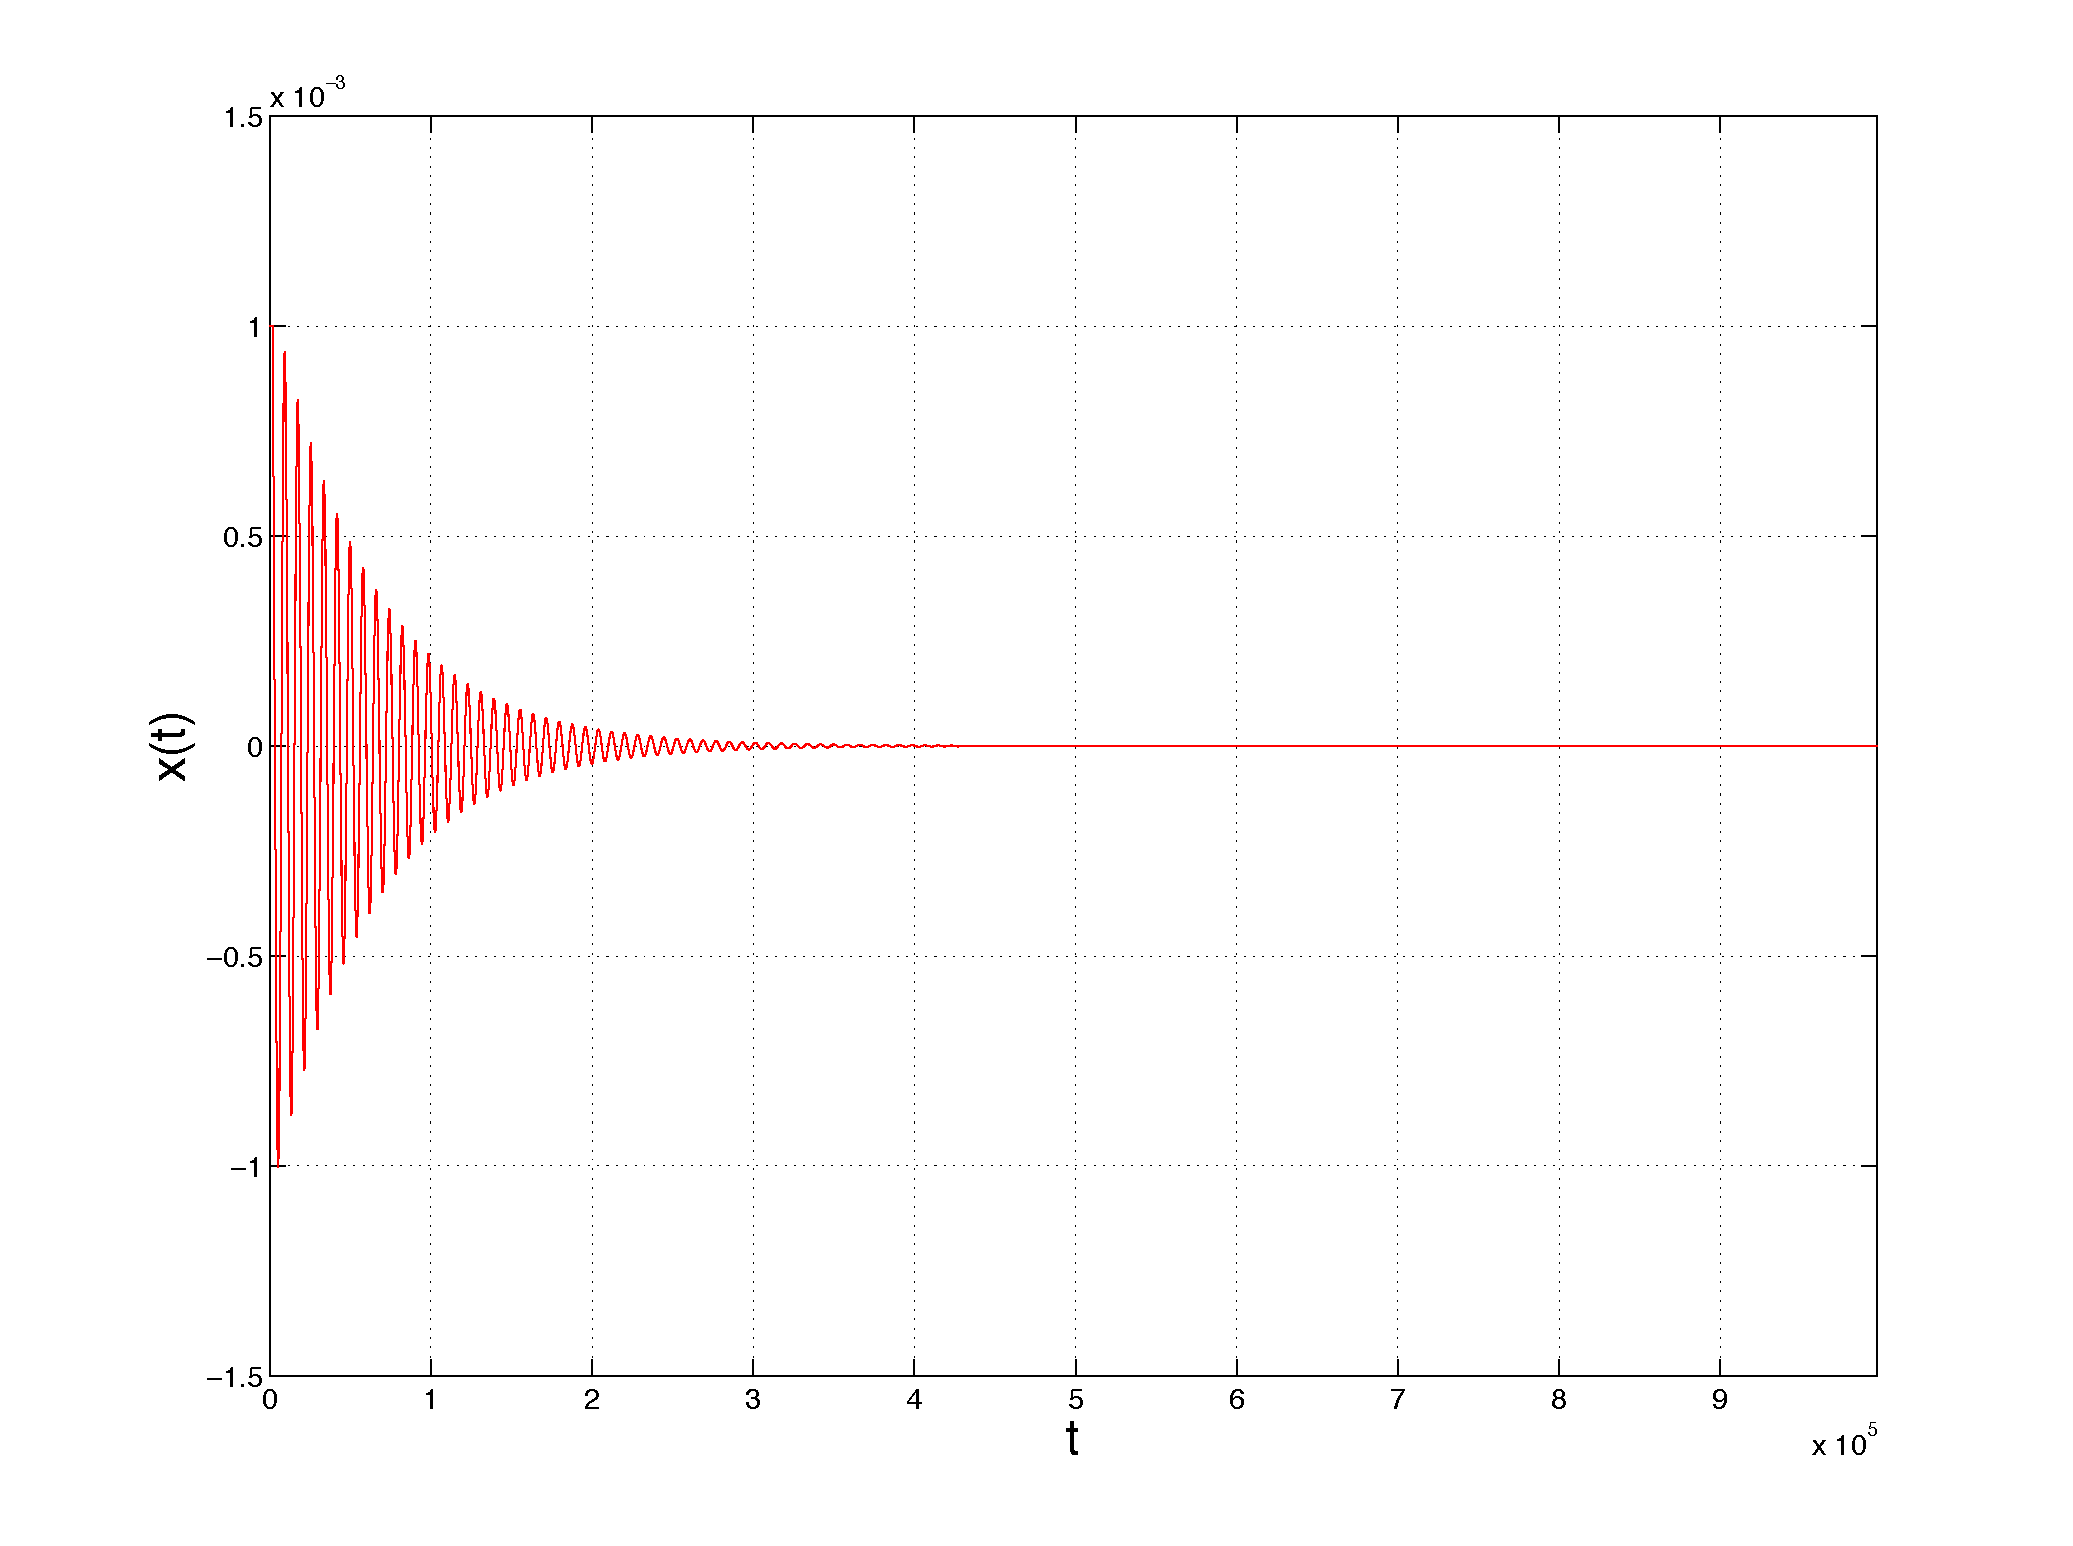
\includegraphics[width=\textwidth]{pso.pdf}
 \caption{The attractivity of $x(t)$ with the largest $r$ satisfying $r(m+1)\leqslant3/2$.}\label{fig2}
\end{figure}
\begin{figure}[!htb]
\centering
 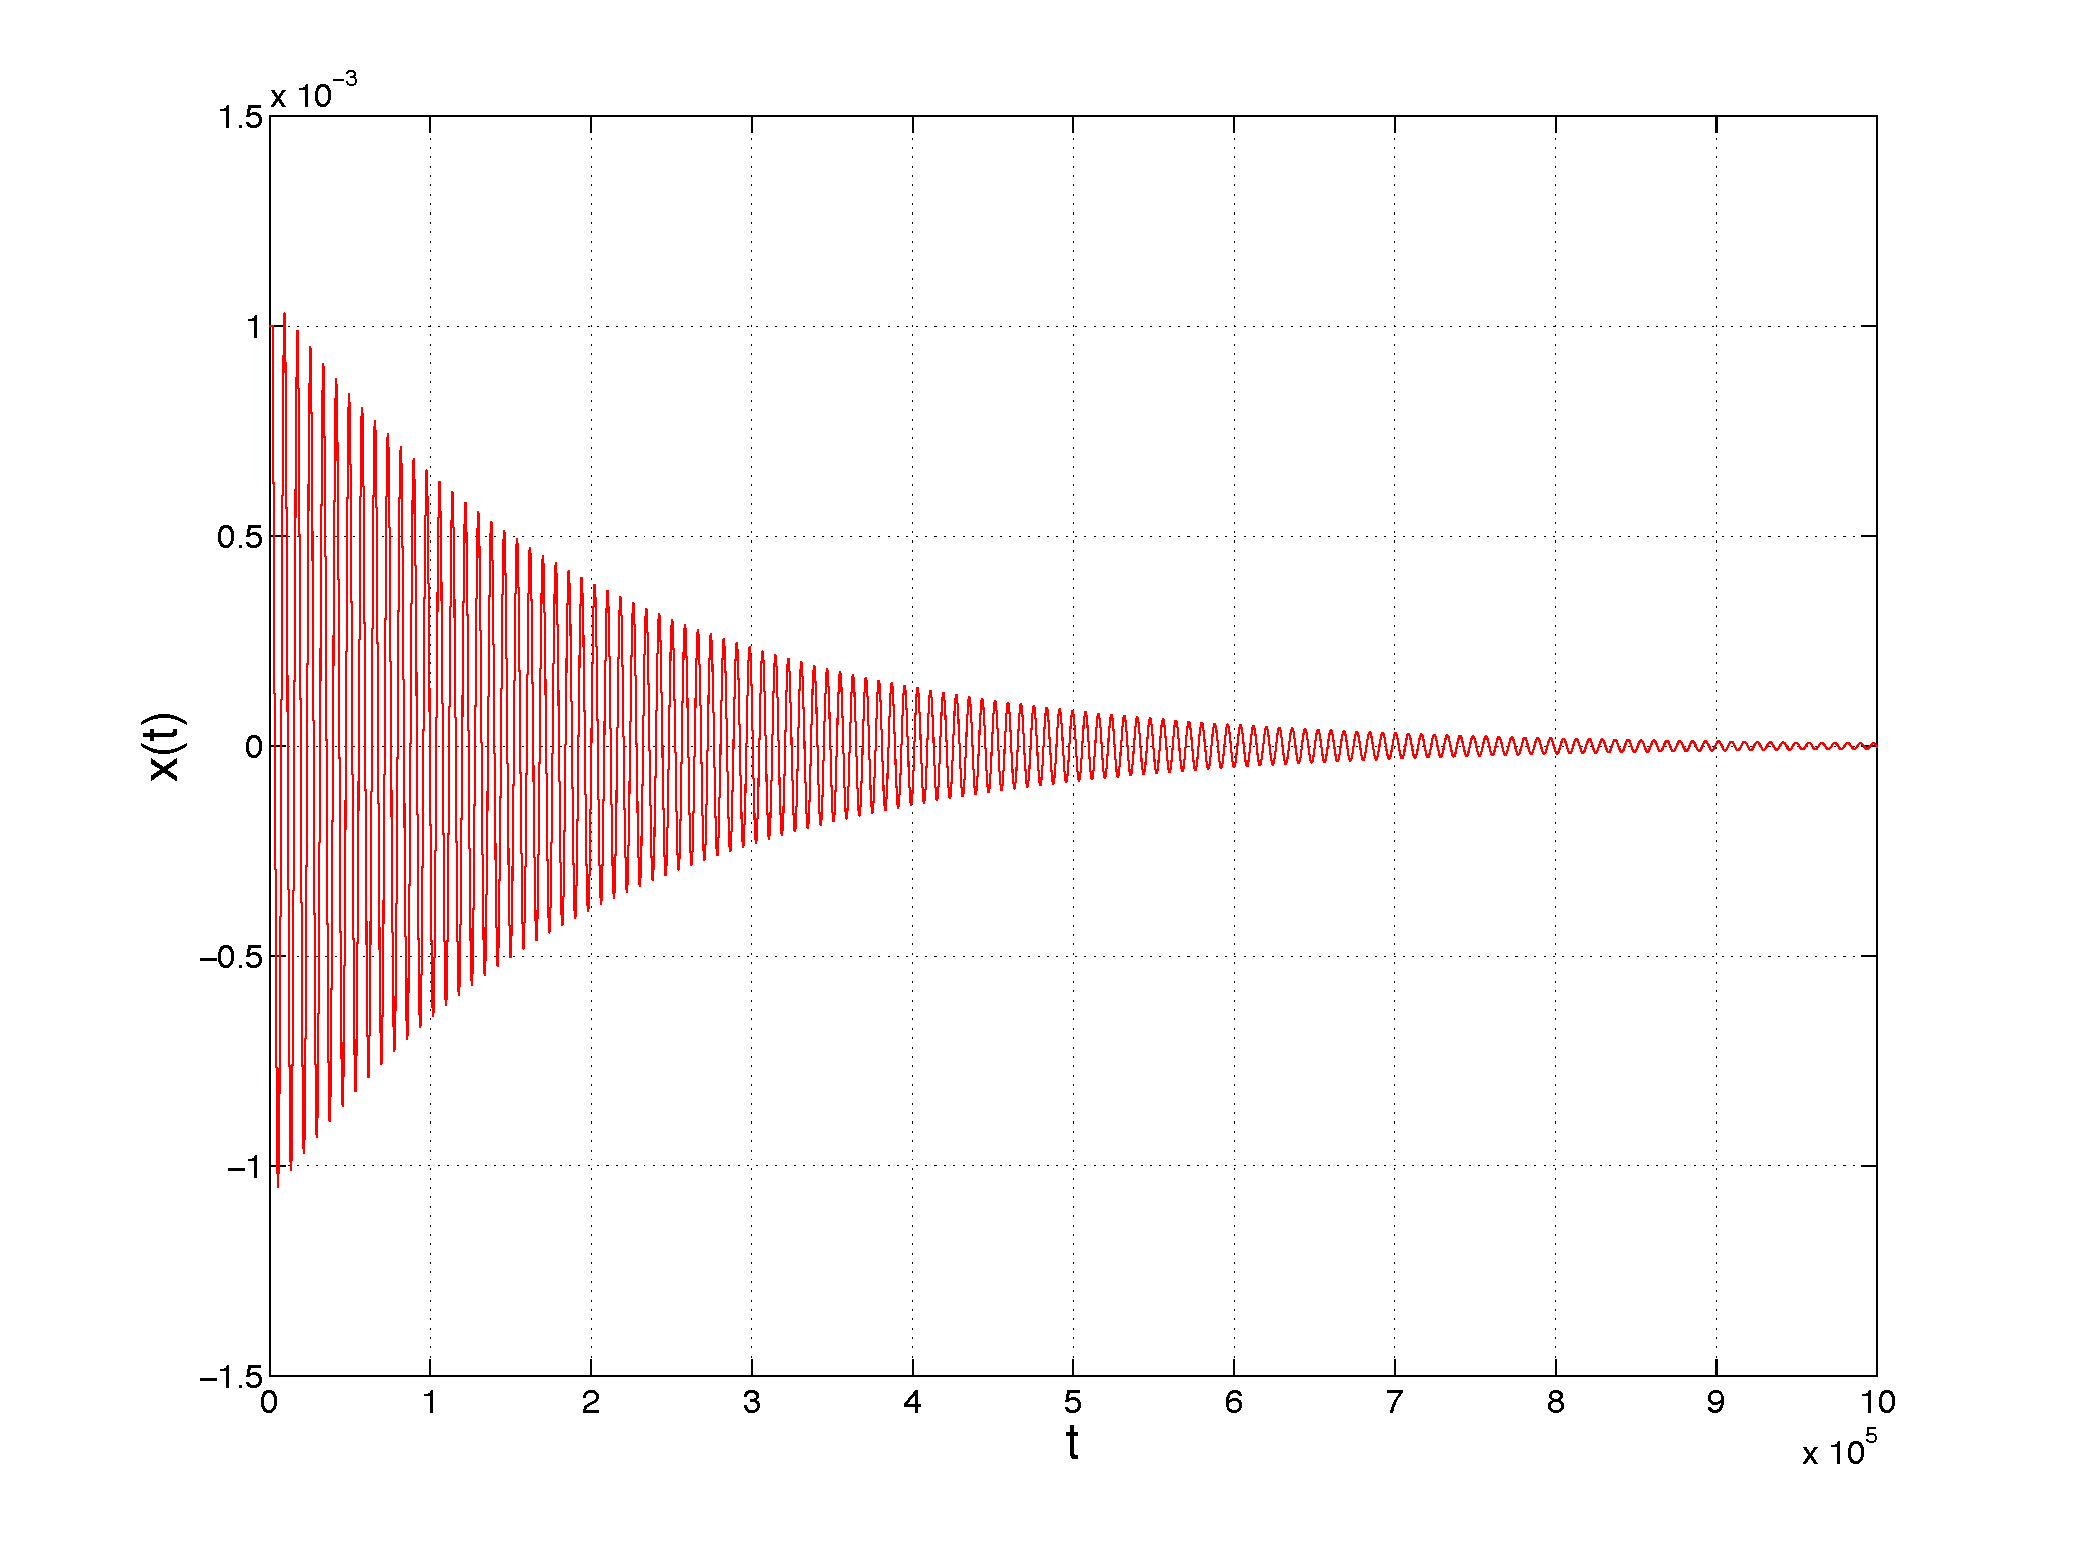
\includegraphics[width=\textwidth]{pour.pdf}
 \caption{The attractivity of $x(t)$ with the largest $r$ satisfying {$r(m+1)-e^{-r(m+1)-1.5}\leqslant3/2$}.}\label{fig3}
\end{figure}

Figure \ref{fig2} and Figure \ref{fig3} show our  computer simulations.
For demonstrating the solution $N(t)$ of \eqref{logistic_equation}-\eqref{logistic_initial_condition}, we simulate the solution $x(t)$ of  \eqref{xt_eq_def}-\eqref{initial_xt_def}  equivalently. We choose
\begin{align*}
&m=2000,  x(0)=x(1)=\cdots=x(m)=0.001,\\
&\alpha_0=\alpha_1=\cdots=\alpha_{m-1}=0,\alpha_m=1
\end{align*}in \eqref{xt_eq_def}-\eqref{initial_xt_def} and $r$ is the largest constant satisfying  \eqref{c2} and \eqref{c3}, respectively. Figure \ref{fig2} and Figure \ref{fig3} are the diagrams of the  solutions $x(t)$ with respect to $t$. Figure \ref{fig2} shows the situation under \eqref{c3}, which stands for So and Yu$'$s condition, while Figure \ref{fig3} shows the situation under \eqref{c2}, which stands for   our condition.  From Figure \ref{fig2} and Figure \ref{fig3}, we   know the larger $r$ is, the slower the convergence rate of $x(t)$ adapts.




\newpage
\begin{table}[!htb]
\begin{small}
\begin{center}
\caption{List of largest $r$ satisfying different conditions \eqref{c1}-\eqref{c4}.}\label{tab1}
\begin{tabular}{l|lllllll}
\hline
$m$&0&1&2&3&4&5&6\\
\hline
 $r_{QuestionA}(m)$&1.570797&0.785399&0.523599&0.392700&0.314160&0.26180&0.224400\\
$r_{Ours}(m)$          &1.547479&0.773740&0.515827&0.386870&0.309496&0.257914&0.221069\\
$r_{So\&Yu}(m)$      &1.500001&0.750000&0.500001&0.375001&0.300001&0.250000&0.214286\\
$r_{Gopalsamy}(m)$&0.567144&0.283572&0.189048&0.141786&0.113429&0.094524&0.081021\\
\hline
\end{tabular}
\end{center}
\end{small}
\end{table}
\newpage
\listoffigures
\newpage
\addcontentsline{toc}{section}{References}
\bibliographystyle{unsrt}%{brief}%{alpha}%{unsrt}
\bibliography{paper}
\end{document}
